\graphicspath{%
{chapter1graph/}%
{chapter1graph/bg/}}
%\makeindex


\chapter{Distribution}

This chapter deals with concepts mainly related to various probability distribution.

\section{Probability Mass Function (PMF)}

The Probability Mass Function (PMF) gives the set of probabilities of \underline{discrete} outcome, e.g. discrete uniform PMF: roll one dice, each outcome is 1/6. \\

More formally, a probability mass function (PMF) is a function that gives the probability that a discrete random variable is exactly equal to some value. In Eqn. (\ref{binomialPMF}) below, the PMF gives the probability of getting exactly $k$ (discrete) successful Bernoulli trails. \\

Formal definition:\\
PMF is the probability distribution of a discrete random variable, and provides the possible values and associated probabilities. The probabilities associated with each possible values must be positive and sum up to 1. For all other values, the probabilities need to be 0.

\begin{figure}[h!]
\begin{center}
	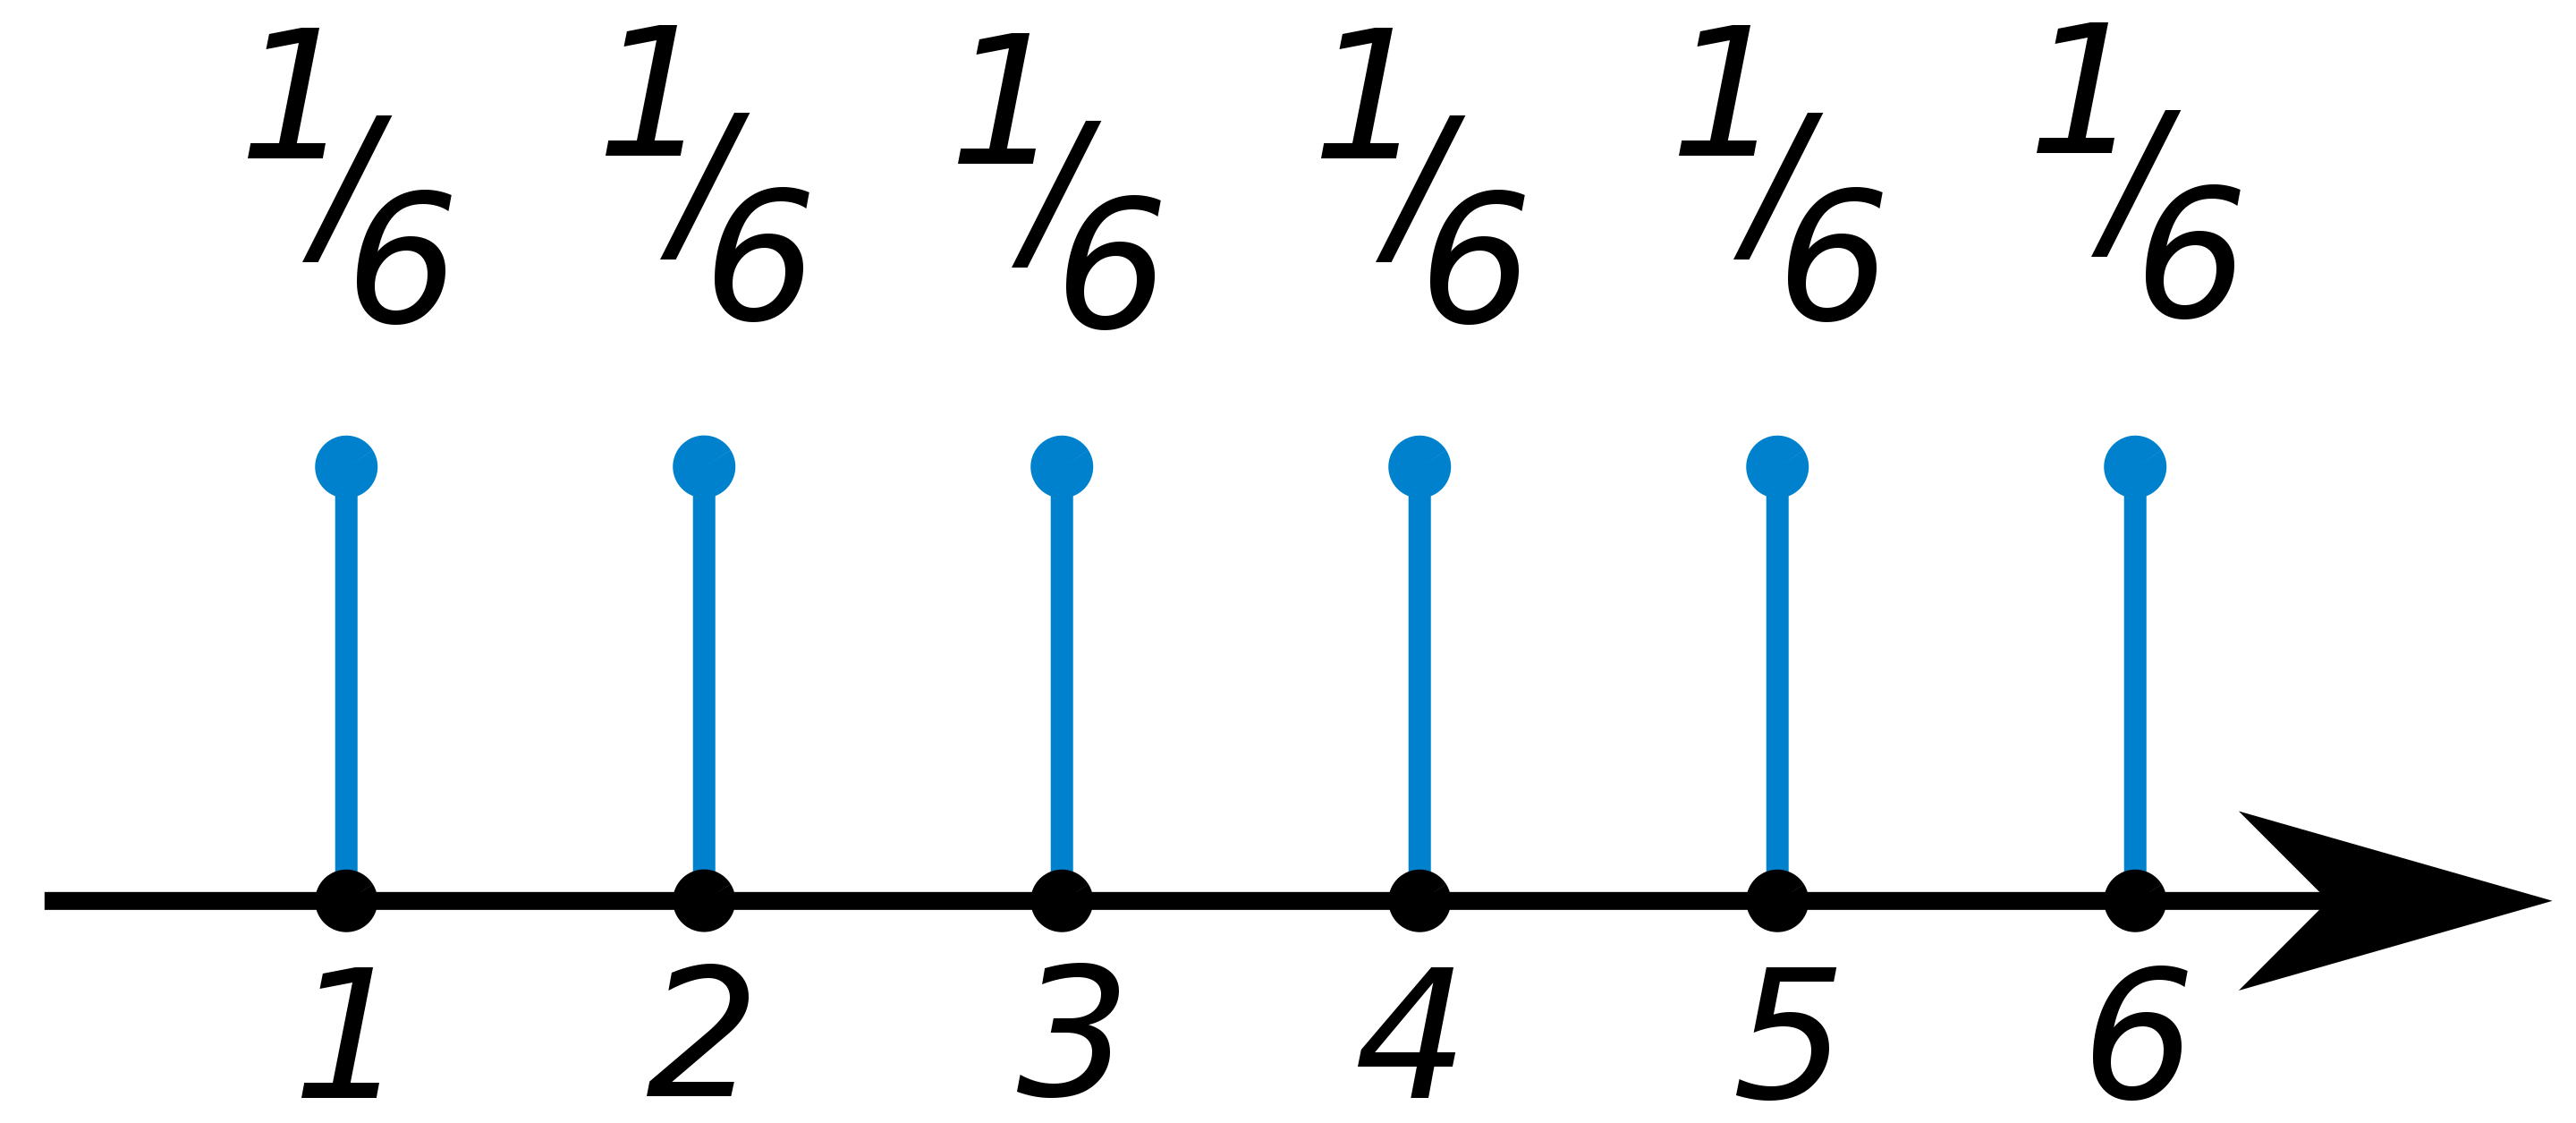
\includegraphics[scale=0.05]{Fair_dice_probability_distribution.png}
	\caption[]{The probability mass function of a fair die. All the values of this function must be non-negative and sum up to 1}
	\label{fairdiepmf}
	\end{center}
	\end{figure}

\section{Probability Density Function (PDF)}

The Probability Density Function (PDF) of a \underline{continuous} random variable, is a function whose value at any given sample (or point) in the sample space (the set of possible values taken by the random variable) can be interpreted as providing a relative likelihood that the value of the random variable would equal that sample. \\

In a more precise sense, the PDF is used to specify the probability of the random variable falling within a particular range of values, as opposed to taking on any one value. This probability is given by the integral of this variable's PDF over that range—that is, it is given by the area under the density function but above the horizontal axis and between the lowest and greatest values of the range. The probability density function is nonnegative everywhere, and its integral over the entire space is equal to 1. A PDF must be integrated over an interval to yield a probability, which is different from PMF (other than continuous VS discrete random variable).\\

More formally, the PDF is most commonly associated with absolutely continuous univariate distribution, a random variable $X$ has PDF $f_X$ and the probability of this variable taking values between $a$ and $b$, i.e. $a \le X \le b$ will be:
\begin{eqnarray}
P(a \le X \le b) = \int^{b}_{a} f_X (x) dx
\label{pdf}
\end{eqnarray}

If $F_X$ is the cumulative distribution function (CDF) of X, then:
\begin{eqnarray}
F_X(x) = \int^{x}_{-\infty} f_X(u) du
\label{cdf}
\end{eqnarray}

\begin{figure}[h!]
\begin{center}
	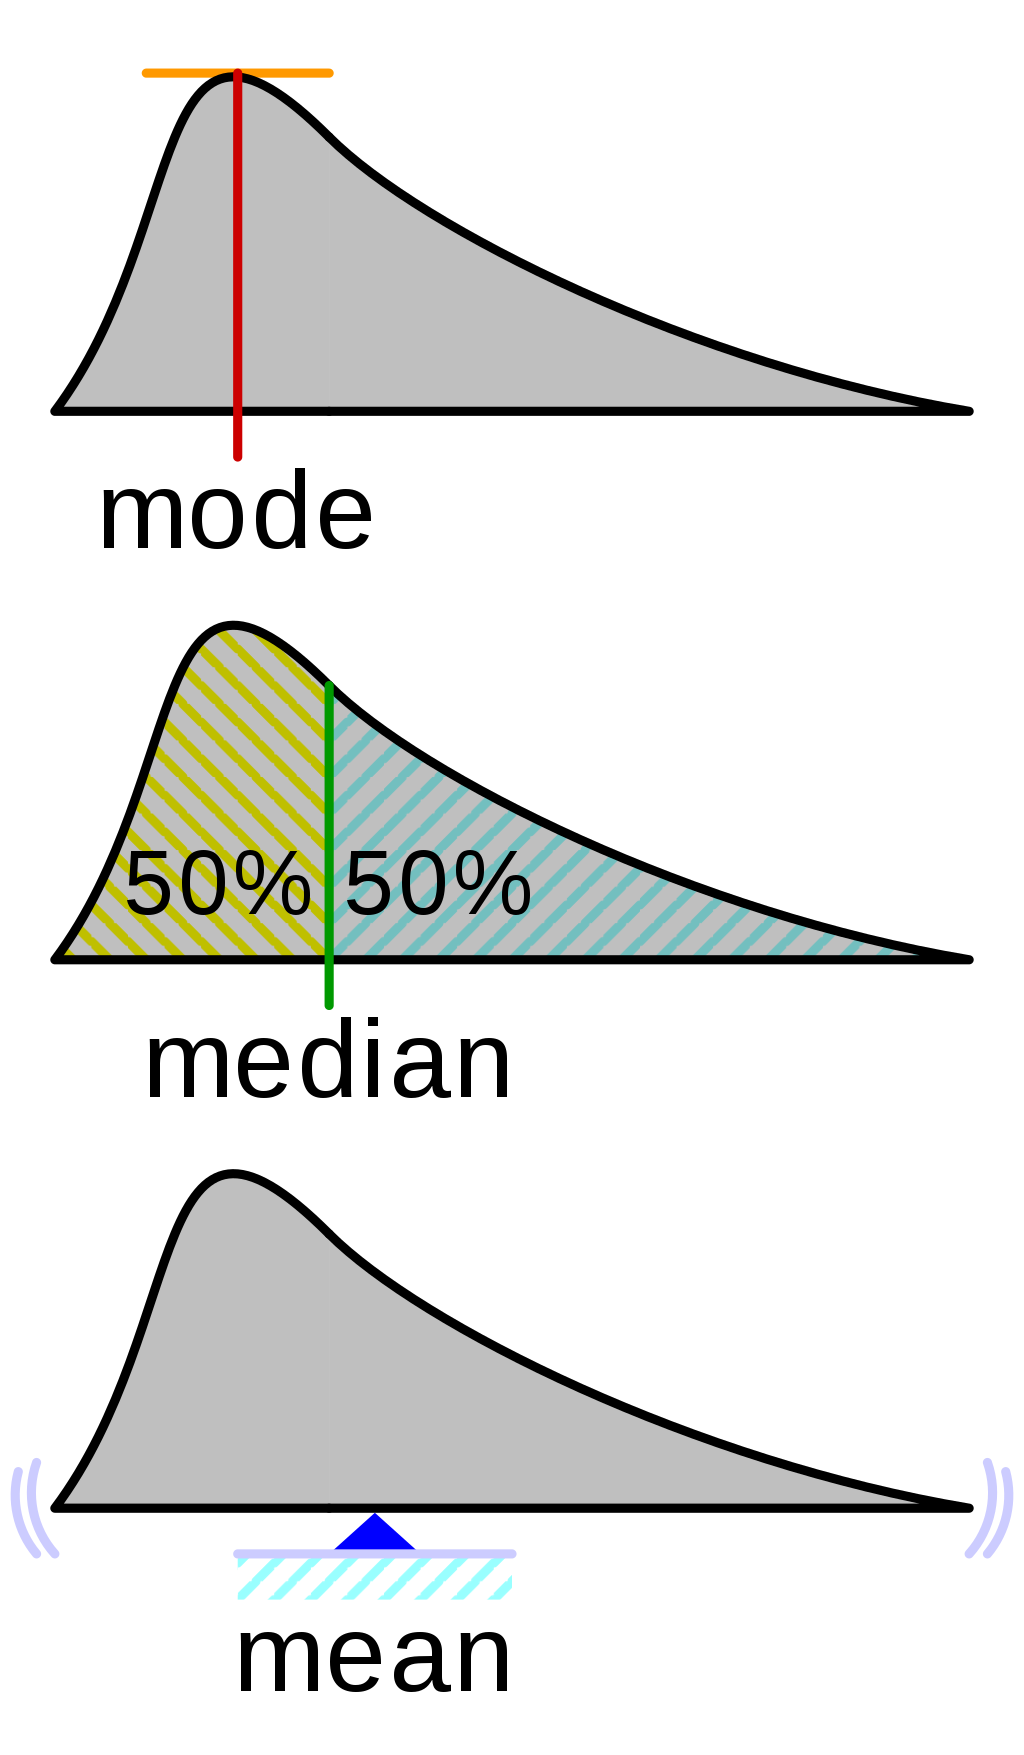
\includegraphics[scale=0.07]{pdf_visual.png}
	\caption[]{Geometric visualisation of the mode, median and mean of an arbitrary probability density function.}
	\label{fairdiepmf}
	\end{center}
	\end{figure}

\section{Cumulative Distribution Function (CDF)}

The Cumulative Distribution Function (CDF) of a real-valued random variable $X$ (continuous or discrete), evaluated at $x$, is the probability that $X$ will take a value less than or equal to $x$. In the case of a scalar continuous distribution, it gives the area under the probability density function (PDF) from $-\infty$ to $x$.

\section{Bernoulli Trials}

This is a \underline{random} experiment with exactly 2 possible outcomes. The probability of success is the same every time experiment is conducted. A similar analogy: Flipping a (possibly) biased coin, each coin has probability \textcolor{blue}{$p$} of landing heads (\textcolor{blue}{success}) and probability \textcolor{red}{$1 - p$} of landing tails (\textcolor{red}{failure}).  \\

Closely related to a Bernoulli trial is a binomial experiment, which consists of a fixed number $n$ of statistically independent Bernoulli trails, each with a probability of success \textcolor{blue}{$p$}, and counts the number of success. The number $k$ of success in $n$ Bernoulli trials is Binomially distributed. The probability of exactly $k$ success (out of $n$) is given by the probability mass function (PMF): 
\begin{eqnarray}
f(k,n,p) = P(k; n.p) =  P(X = k) = \binom{n}{k} p^k (1-p)^{n-k}
\label{binomialPMF}
\end{eqnarray}
where $\binom{n}{k}$ is the binomial coefficient:
\begin{eqnarray}
\binom{n}{k} = \frac{n !}{k! (n-k)!}
\label{binomialcoef}
\end{eqnarray}

Example:\\
Let's say a bank made 100 mortgage loans. It is possible that anywhere between 0 and 100 of the loans will be defaulted upon. You would like to know the probability of getting a given number of defaults, given that the probability of a default is $p = 0.05$. To investigate this, you will do a simulation. You will perform 100 Bernoulli trials. Here, a success is a default. (Remember that the word `success' just means that the Bernoulli trial evaluates to be True, i.e., did the loan recipient default?) You will do this for another 100 Bernoulli trials. And again and again until we have tried it 1000 times. Then, you will plot a histogram describing the probability of the number of defaults. So we have performed 1000 times of 100 mortgage trials, the histogram should show a maximum at about 5 (because $0.05 \times 100$) and probability is given in Eqn. (\ref{binomialPMF}). \\   

Example:\\
Consider the simple experiment where a fair coin is tossed four times. Find the probability that exactly two of the tosses result in heads.\\
\begin{eqnarray*}
P(2) &=& \binom{4}{2}p^2 (1-p)^{4-2} \\ 
&=& 6 \times (0.5)^2 \times (0.5)^2 \\ 
&=& \frac{3}{8}\\ 
\label{coin}
\end{eqnarray*}

When multiple Bernoulli trials are performed, each with its own probability of success, these are sometimes referred to as Poisson trials.

\section{Discrete variable: Binomial Distribution}

The Binomial Distribution with parameters $n$ and $p$, denoted Bin$(n,p)$ is the discrete probability distribution of the number of successes in a sequence of $n$ independent experiments, each asking a yes–no question, and each with its own boolean-valued outcome True (with probability $p$), or failure (with probability $q = 1- p$). A single success or failure experiment is also called a Bernoulli trial. \\

The binomial distribution is frequently used to model the number of successes in a sample of size $n$ drawn with replacement from a population of size $N$. If the sampling is carried out without replacement, then the draws are not independent and so the resulting distribution would be a hypergeometric distribution, not a binomial one. However, for N much larger than n, the binomial distribution remains a good approximation, and is widely used.

The PMF of Binomial Distribution is given in Eqn.(\ref{binomialPMF}). The CDF of Binomial Distribution can be expressed as:
\begin{eqnarray}
F(k; n, p) = P (X \le k) = \sum_{i=0}^{k} \binom{n}{i} p^i (1-p)^{n-i}
\label{binomialCDF}
\end{eqnarray}
where we just add up all the probability for all the previous $k$ values.

\section{Discrete variable: Bernoulli distribution}
The Bernoulli distribution is a special case of the binomial distribution, where a single trial is conducted (i.e., a binomial distribution with $n = 1$). The PMF of Bernoulli distribution, over possible outcomes $j$ is:
\begin{eqnarray}
f(k;p) = \begin{cases}
p,             \text{if $j$ = 1}\\
q = 1-p,      \text{if $j$ = 0}
\end{cases}
\end{eqnarray}

\section{Discrete variable: Geometric Distribution}

The Geometric Distribution is either of two discrete probability distribution described below: \\

1) The probability distribution of the number $X$ of Bernoulli Trials 

\section{Discrete variable: Poisson Distribution}

\section{Continuous variable: Normal/Gaussian Distribution}

\section{Continuous variable: Exponential Distribution}



